\newcommand{\Screenshot}[1]{%
  \fbox{%
    \begin{minipage}[c][9cm][c]{0.42\textwidth}%
      \centering\small\color{gray!60}[snímek obrazovky: #1]%
    \end{minipage}%
  }%
}

\chapter*{Výsledky}
\addcontentsline{toc}{chapter}{Výsledky}

Výsledkem projektu je funkční mobilní aplikace LifeMeter
dostupná na operačních systémech Android (verze 10 a vyšší),
doplněná o~serverový backend a~webovou vrstvu nasazené na doméně
\texttt{lifemeter.fit}. Webová část poskytuje veřejnou prezentaci,
verzované centrum stahování mobilních buildů a~administrátorskou
konzoli pouze pro čtení.

% ------------------------------------------------------------------
\section{Splnění požadavků zadání}
% ------------------------------------------------------------------

Následující tabulka uvádí přehled všech požadavků vymezených v~zadání
maturitního projektu a jejich stav po dokončení implementace.

\begin{table}[H]
  \centering
  \caption{Přehled plnění požadavků zadání}
  \label{tab:pozadavky}
  \begin{tabularx}{\textwidth}{|p{5.5cm}|p{1.8cm}|L|}
    \hline
    \textbf{Požadavek} & \textbf{Stav} & \textbf{Poznámka} \\
    \hline
    Záznam fyzických aktivit & splněno
      & Aktivní tréninky se sadami, opakováními a~váhou;
        tréninkové šablony s~přetahováním cvičení. \\
    \hline
    Přidávání potravin, sledování kalorií a~makroživin & splněno
      & Textové vyhledávání i~skenování čárového kódu;
        přehled bílkovin, sacharidů a~tuků za aktuální den. \\
    \hline
    Sledování mikroživin a~vitamínů & splněno
      & Přehled všech mikronutrientů (vitamíny, minerály)
        dostupný přes rozbalovací panel. \\
    \hline
    Záznam délky spánku s~poznámkou & splněno
      & Ruční zadání spánku i~spuštění/ukončení v~reálném čase;
        volitelná textová poznámka ke každému záznamu. \\
    \hline
    Přihlašování e-mailem se zabezpečeným ověřením & splněno
      & Registrace a~přihlášení prostřednictvím knihovny
        Better Auth; relace na bázi bezpečných HTTP cookies. \\
    \hline
    Offline režim se synchronizací & splněno
      & Mutační požadavky jsou při absenci připojení
        ukládány do fronty MMKV a~odeslány po jeho obnovení. \\
    \hline
    Notifikace ke cvičení a~spánku & splněno
      & Konfigurovatelná denní upozornění na čas cvičení,
        dobu uložení ke spánku a~čas vstávání. \\
    \hline
    Integrace s~jinou aplikací/platformou & splněno
      & Health Connect (Android) a~Apple HealthKit (iOS):
        kroky, spánek, váha, výška, spálené kalorie. \\
    \hline
  \end{tabularx}
\end{table}

% ------------------------------------------------------------------
\section{Implementované moduly}
% ------------------------------------------------------------------

Aplikace je rozdělena do pěti hlavních funkčních modulů přístupných
přes spodní navigační lištu.

\textbf{Onboarding} provádí nového uživatele čtyřkrokovým průvodcem:
zadání základních údajů (pohlaví, datum narození, preferované
jednotky), tělesných měr (výška, váha, případně procento tělesného
tuku), úrovně pohybové aktivity a~cílů (cílová váha, datum dosažení,
denní kroky, časy spánku). Z~těchto vstupů je vypočítán bazální
metabolismus metodou Mifflin–St~Jeor a~z~něj odvozeny personalizované
makronutrientní cíle.

\textbf{Domovská obrazovka} zobrazuje přehledový dashboard za
posledních 7~dní: sloupcový graf denních kroků synchronizovaný
z~platformy zdravotních dat, kalorický graf výživy, přehled doby
spánku a~graf tréninkové aktivity.

\textbf{Modul výživy} umožňuje přidávání jídel textovým vyhledáváním
v~databázi přes 1~000~000 potravin ze zdroje USDA FoodData
Central nebo skenováním čárového kódu EAN-13/EAN-8/UPC. Denní makra
jsou zobrazena graficky jako okruháčové grafy s~absolutními hodnotami
a~procentuálním plněním cíle. Přehled mikronutrientů je dostupný
prostřednictvím vysunovacího panelu.

\textbf{Modul spánku} uchovává historii spánkových záznamů a~umožňuje
spuštění spánkové relace v~reálném čase nebo ruční zadání časového
rozmezí. Na zařízeních se zdravotní platformou jsou automaticky
importovány historické záznamy spánkových fází (bdění, lehký spánek,
hluboký spánek, REM).

\textbf{Modul tréninku} nabízí správu tréninkových šablon s~možností
přetahování pořadí cvičení a~zaznamenávání aktivního tréninku
s~běžícím časovačem. Grafy průběhu výkonu u~jednotlivých cvičení
sledují maximální váhu, odhadnuté maximum pro jedno opakování
(1RM) dle Epleyho vzorce a~celkový tréninkový objem.

\textbf{Nastavení} (přístupné z~hlavičky aplikace) sdružuje správu
profilu a~cílů, konfiguraci oznámení, přepínač offline režimu,
propojení s~platformou zdravotních dat a~přepínač světlého
a~tmavého motivu.

Mimo samotnou mobilní aplikaci byla implementována také \textbf{veřejná
webová vrstva}, která prezentuje produkt, zpřístupňuje aktuální i~
archivní mobilní buildy a~sjednocuje distribuční odkazy. Na stejné
doméně běží rovněž \textbf{administrátorská konzole pouze pro čtení},
určená pro kontrolu systémového přehledu, logů a~detailů uživatelských
účtů.

% ------------------------------------------------------------------
\section{Technické parametry}
% ------------------------------------------------------------------

\begin{table}[H]
  \centering
  \caption{Přehled technických parametrů aplikace}
  \label{tab:technicke-parametry}
  \begin{tabularx}{\textwidth}{|p{6.5cm}|L|}
    \hline
    \textbf{Parametr} & \textbf{Hodnota} \\
    \hline
    Podporované platformy
      & Android 10+, iOS 16+ \\
    \hline
    Počet obrazovek (navigačních uzlů)
      & 10 (4 hlavní záložky, onboarding, aktivní trénink,
        sestavení šablony, seznam spánku, přihlášení, registrace) \\
    \hline
    Počet webových rout
      & 8 (landing page, download centrum, admin login,
        forbidden, dashboard, logy, uživatelé, detail uživatele) \\
    \hline
    Počet REST API endpointů
      & 52 explicitně definovaných + \texttt{/api/auth/*} \\
    \hline
    Počet databázových tabulek
      & 37 dokumentovaných tabulek (33 aplikačních + 4 autentizační Better Auth) \\
    \hline
    Počet potravin v databázi
      & přes 1~000~000 (zdroj USDA FoodData Central, CC0~1.0) \\
    \hline
    Počet sledovaných nutrientů na potravinu
      & až 150 (makronutrienty, vitamíny, minerály) \\
    \hline
    Fulltextový index vyhledávání
      & PostgreSQL \texttt{tsvector} + GIN index + pg\_trgm \\
    \hline
    Prostředí nasazení
      & Oracle Cloud Infrastructure (ARM),
        Docker Compose (\texttt{db}, \texttt{api}, \texttt{web}),
        Caddy reverzní proxy, TLS \\
    \hline
    Průběžné nasazení
      & GitHub Actions (\texttt{deploy.yml} pro stack,
        \texttt{app-apk.yml} pro vydání APK) \\
    \hline
    Zdravotní integrace
      & Health Connect (Android), Apple HealthKit (iOS) \\
    \hline
    Sledované zdravotní metriky
      & kroky, spánek (fáze), váha, výška, spálené kalorie \\
    \hline
  \end{tabularx}
\end{table}

% ------------------------------------------------------------------
\section{Uživatelské rozhraní}
% ------------------------------------------------------------------

Následující snímky obrazovek dokumentují výslednou podobu aplikace.
Aplikace podporuje světlý i~tmavý motiv; zobrazené snímky zachycují
tmavý motiv.

\begin{figure}[H]
  \centering
  \begin{minipage}{0.46\textwidth}
    \centering
    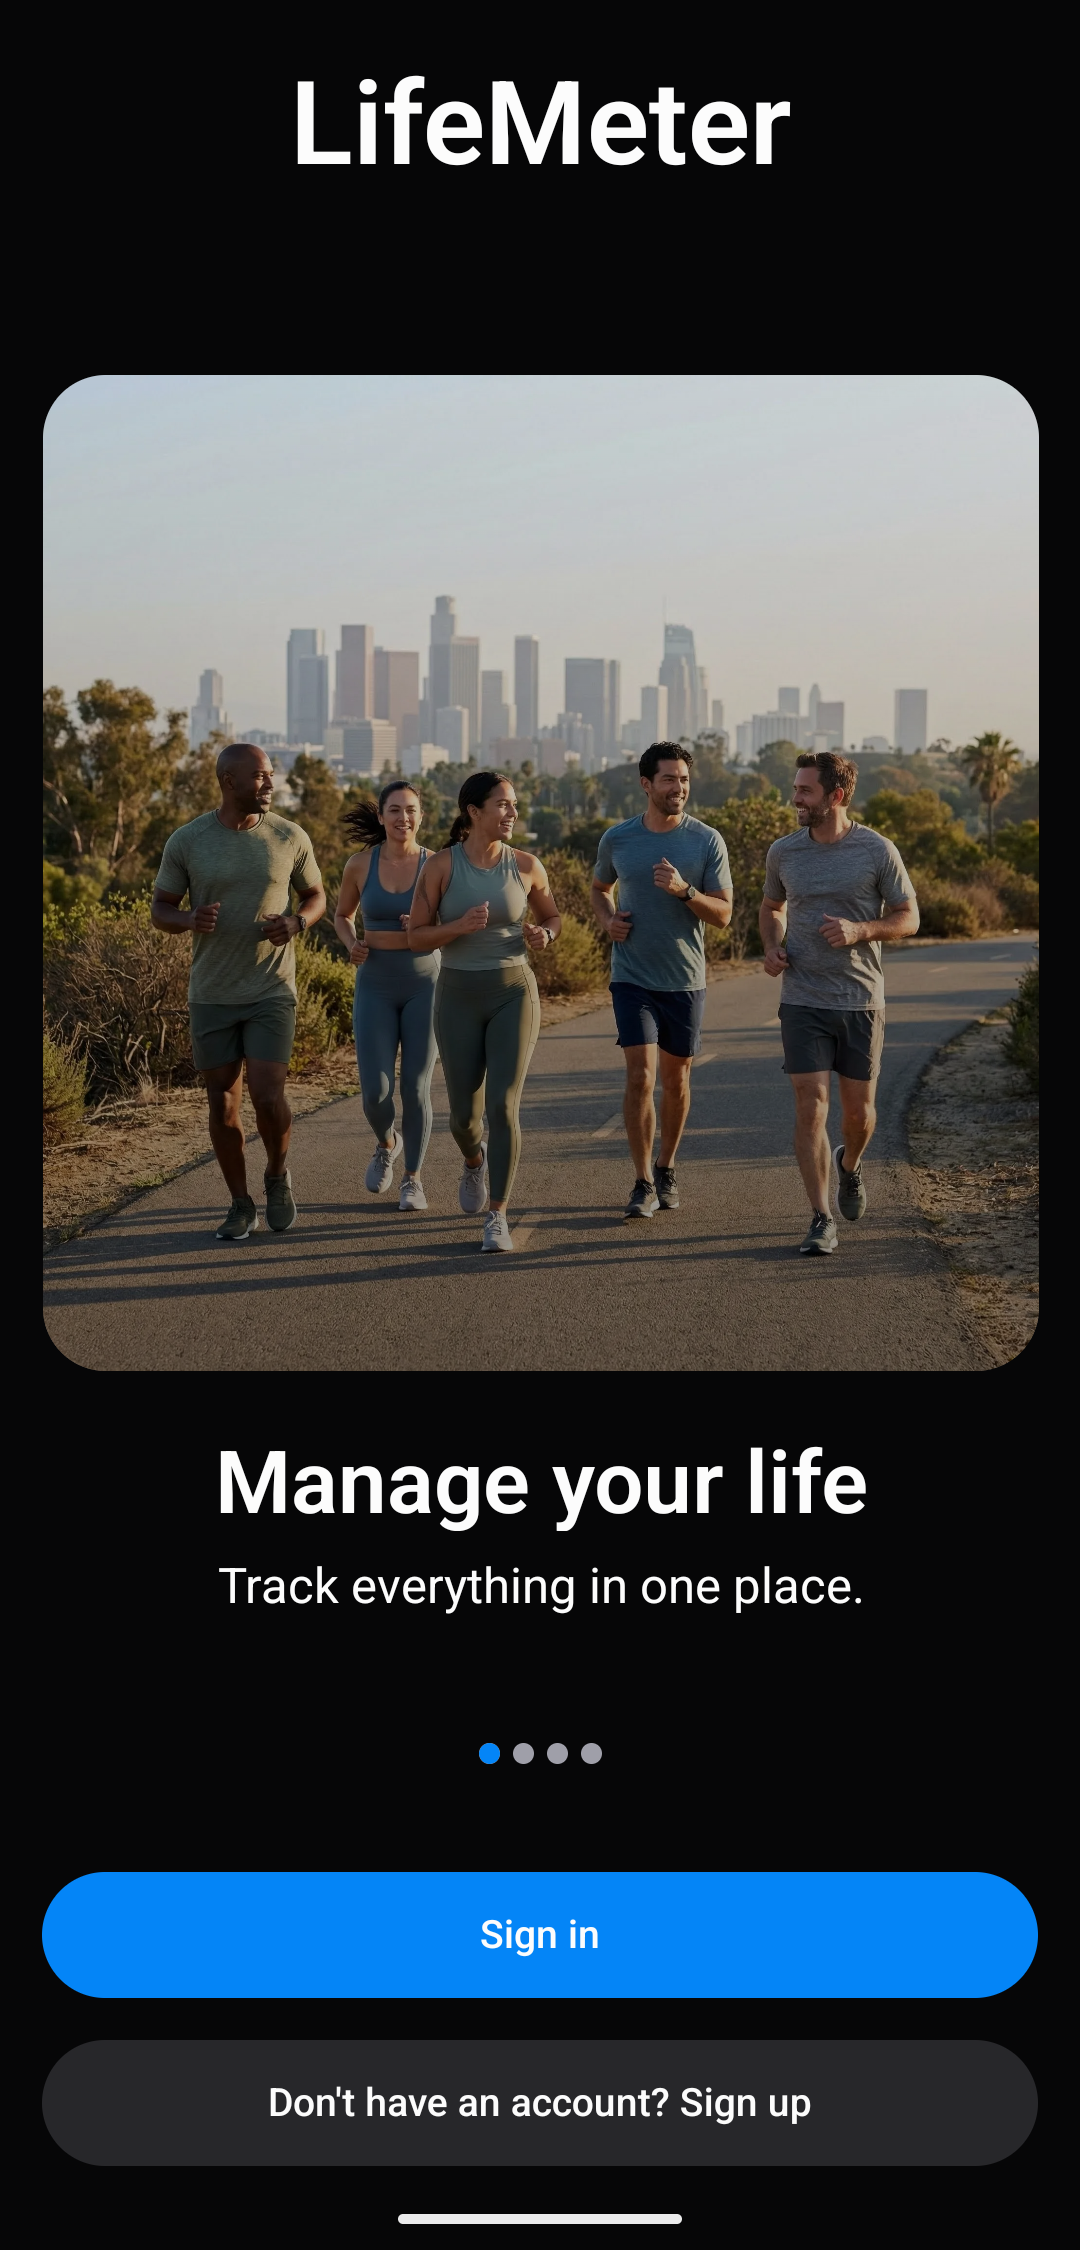
\includegraphics[width=\textwidth]{asset/img/screens/onboarding.png}
    % \Screenshot{onboarding.png}
    \caption{Uvítací obrazovka onboardingu}
    \label{fi g:screen-onboarding}
  \end{minipage}
  \hfill
  \begin{minipage}{0.46\textwidth}
    \centering
    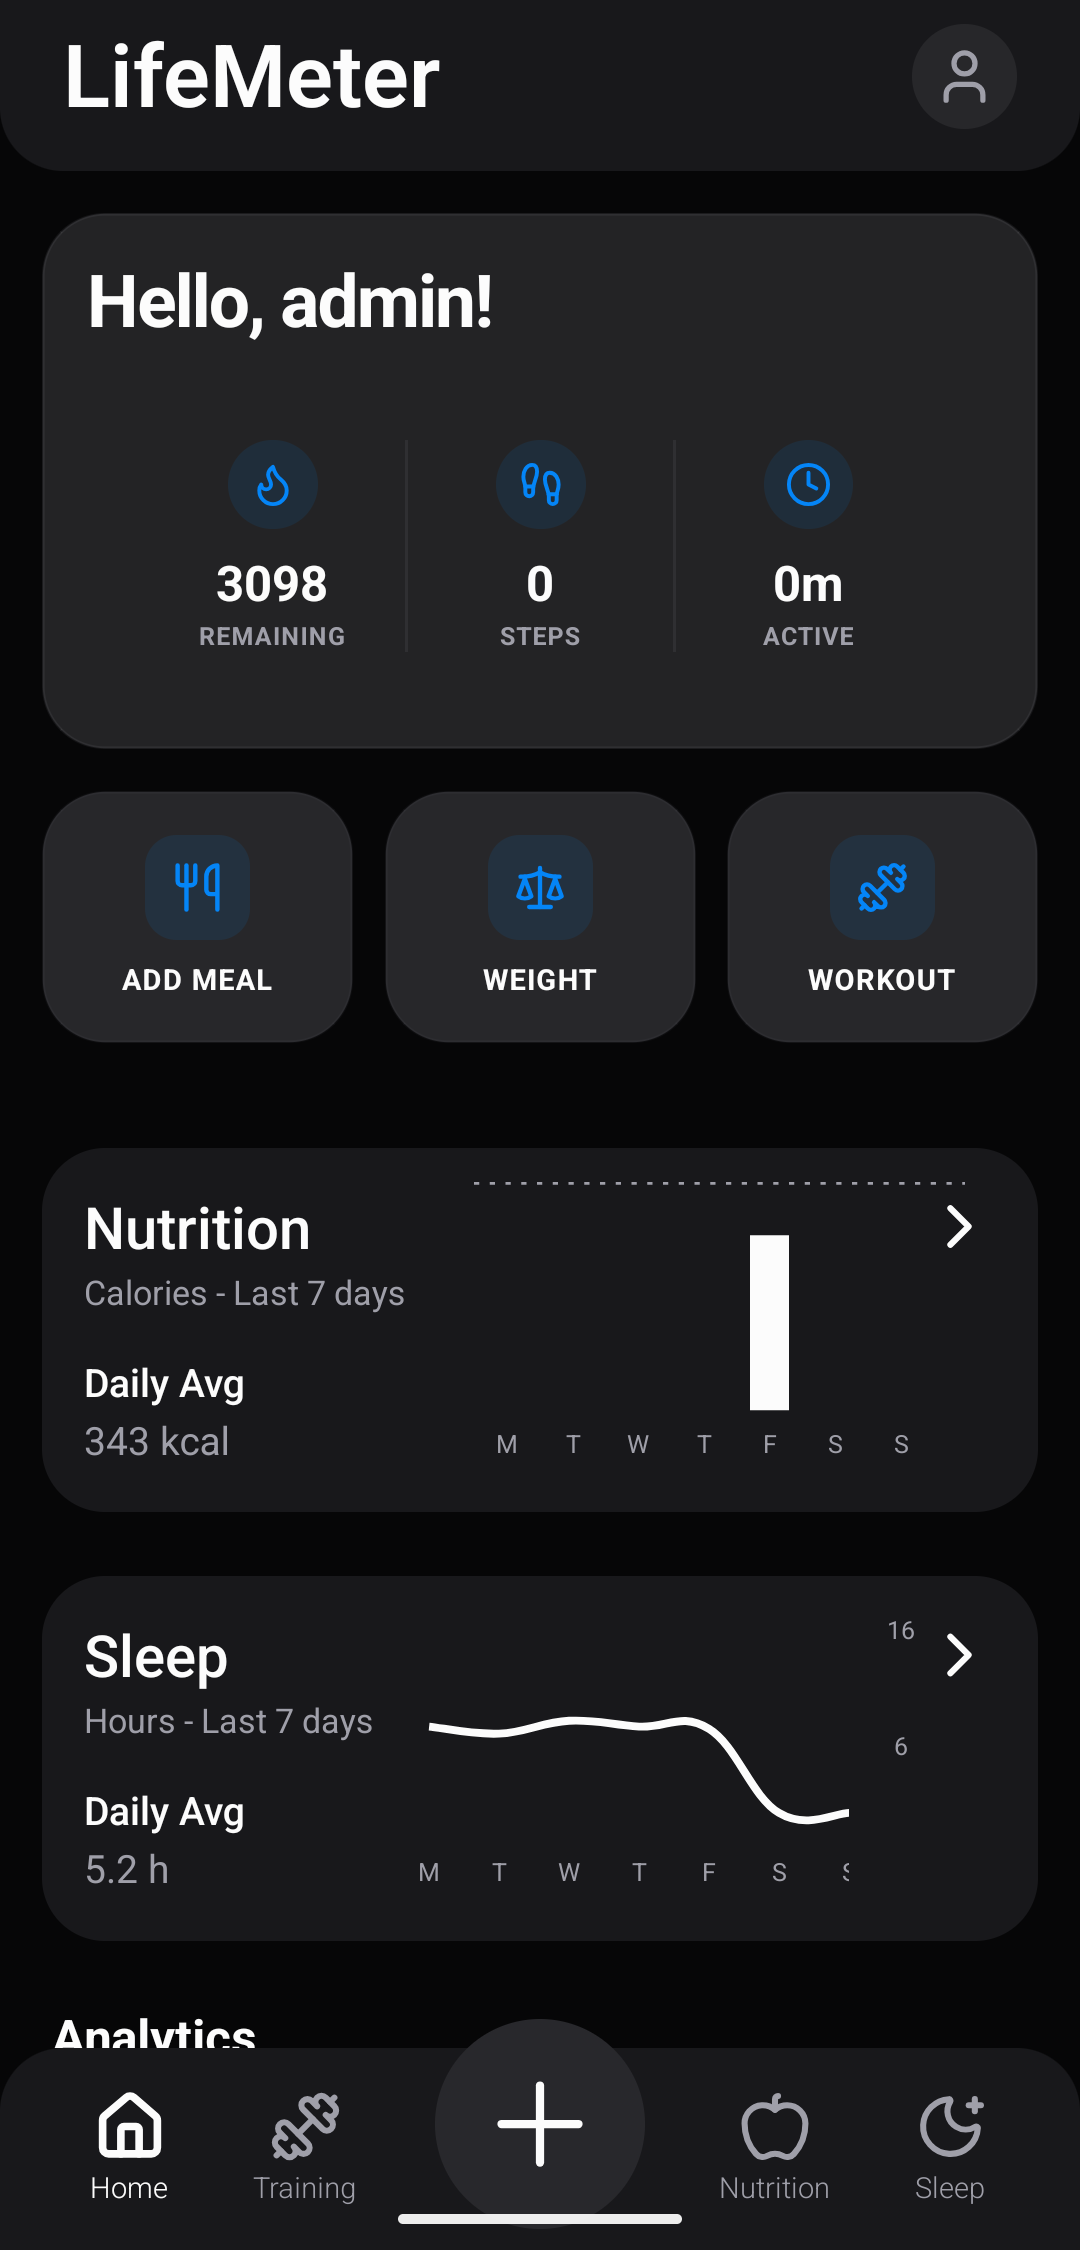
\includegraphics[width=\textwidth]{asset/img/screens/home.png}
    % \Screenshot{home.png}
    \caption{Domovská obrazovka -- 7denní přehled}
    \label{fig:screen-home}
  \end{minipage}
\end{figure}

\begin{figure}[H]
  \centering
  \begin{minipage}{0.46\textwidth}
    \centering
    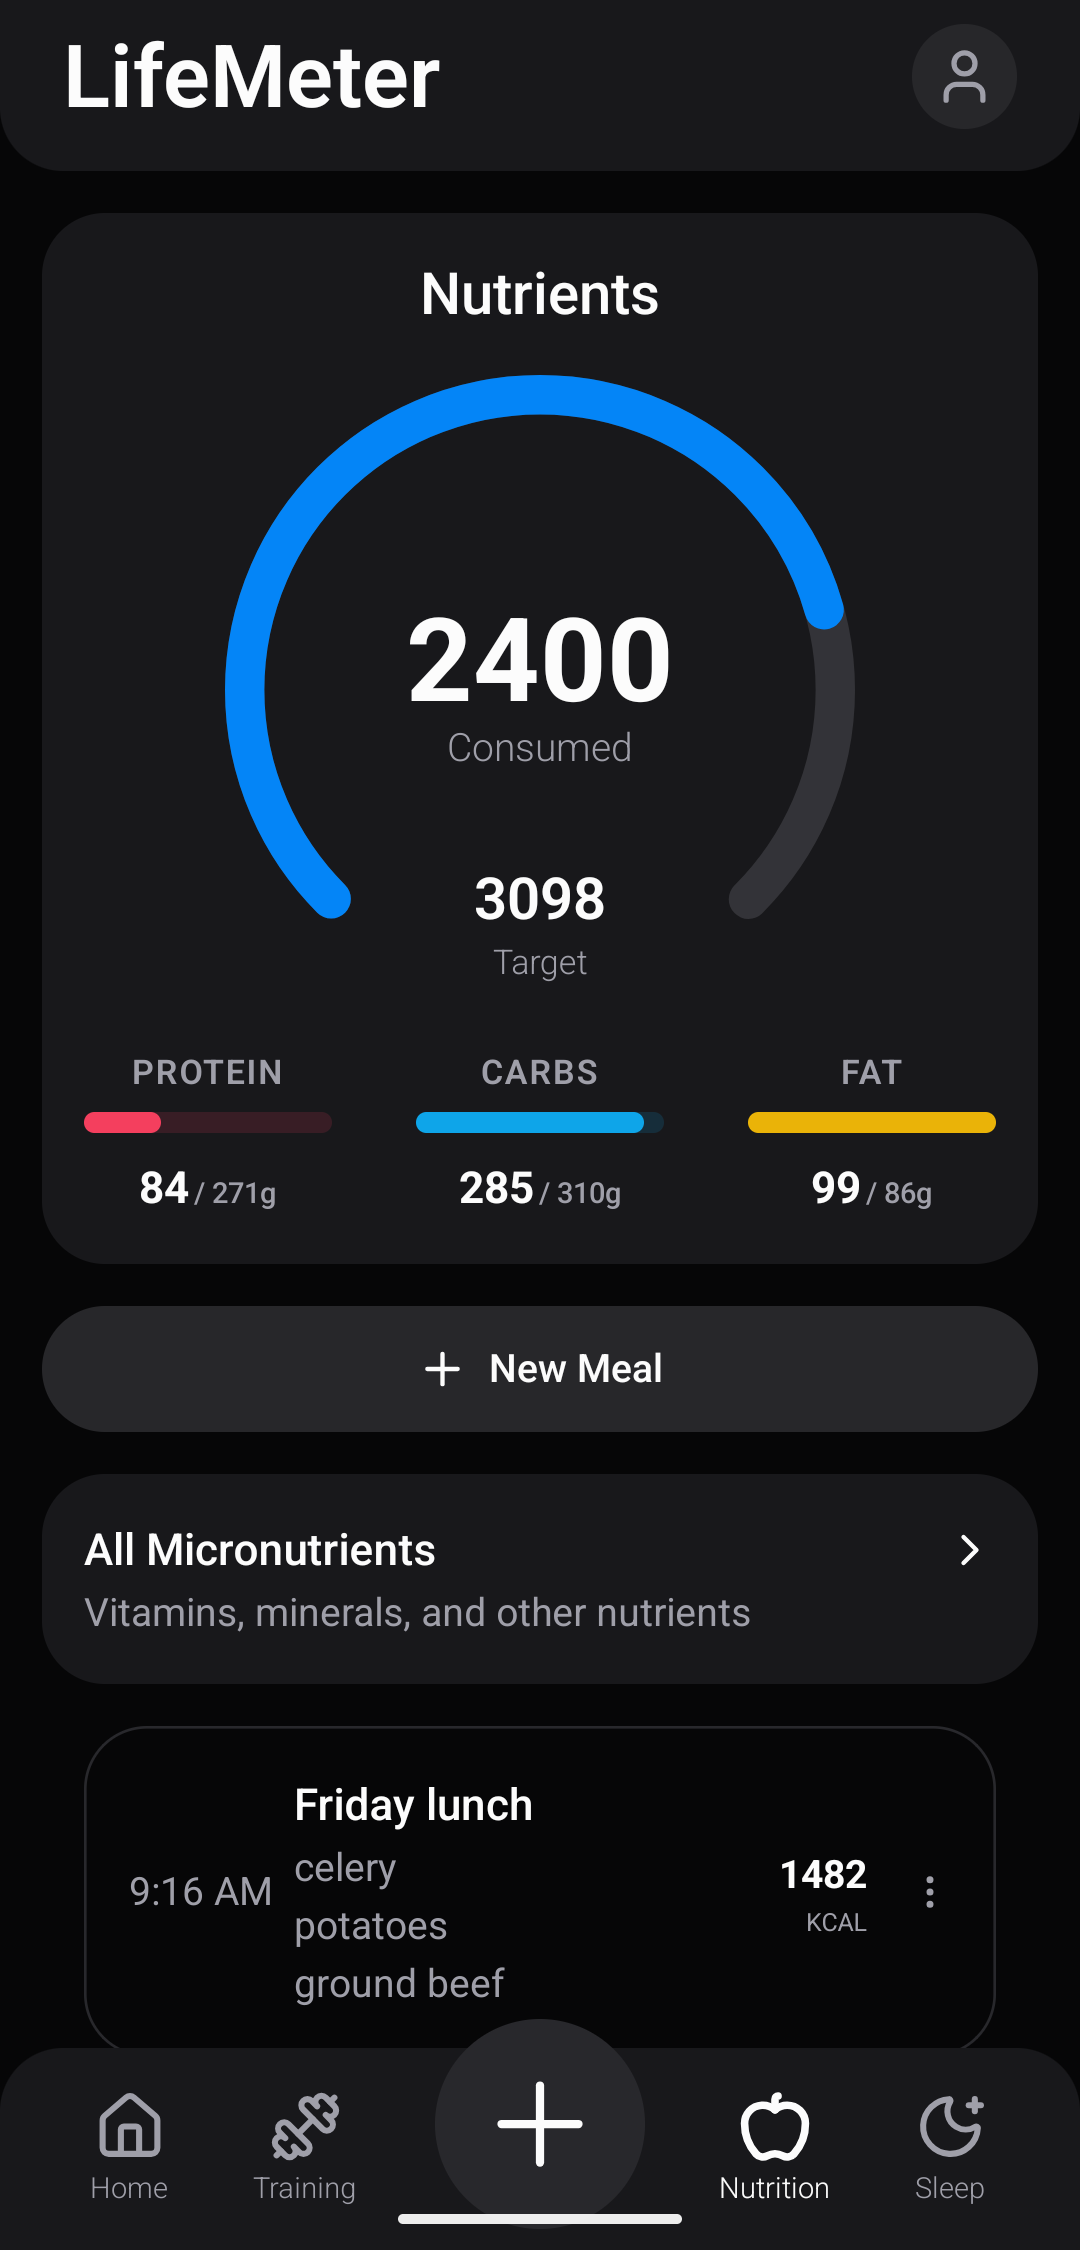
\includegraphics[width=\textwidth]{asset/img/screens/nutrition.png}
    % \Screenshot{nutrition.png}
    \caption{Modul výživy -- denní makra a~přehled jídel}
    \label{fig:screen-nutrition}
  \end{minipage}
  \hfill
  \begin{minipage}{0.46\textwidth}
    \centering
    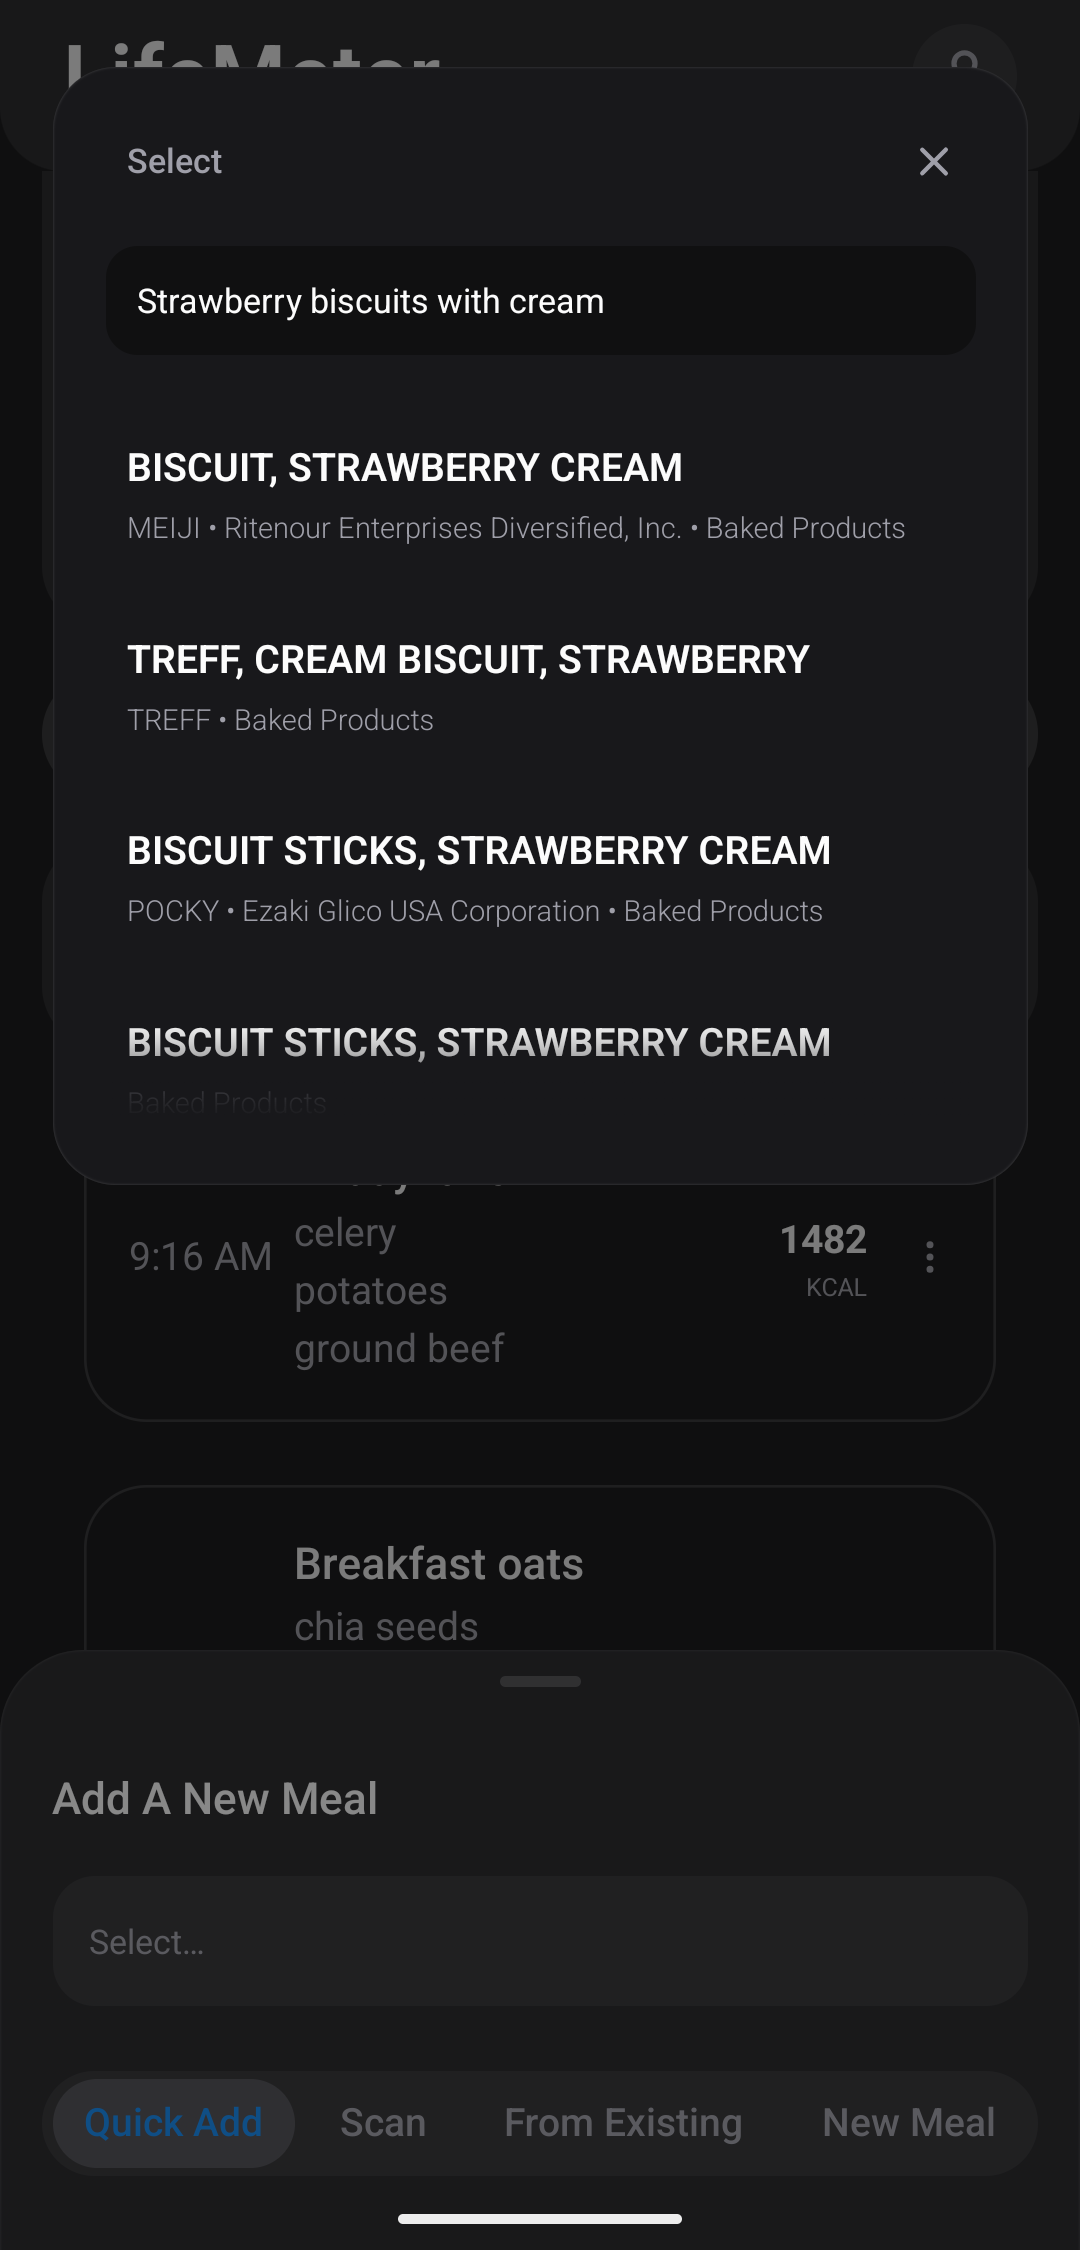
\includegraphics[width=\textwidth]{asset/img/screens/food-search.png}
    % \Screenshot{food-search.png}
    \caption{Vyhledávání potravin a~skenování čárového kódu}
    \label{fig:screen-food-search}
  \end{minipage}
\end{figure}

\begin{figure}[H]
  \centering
  \begin{minipage}{0.46\textwidth}
    \centering
    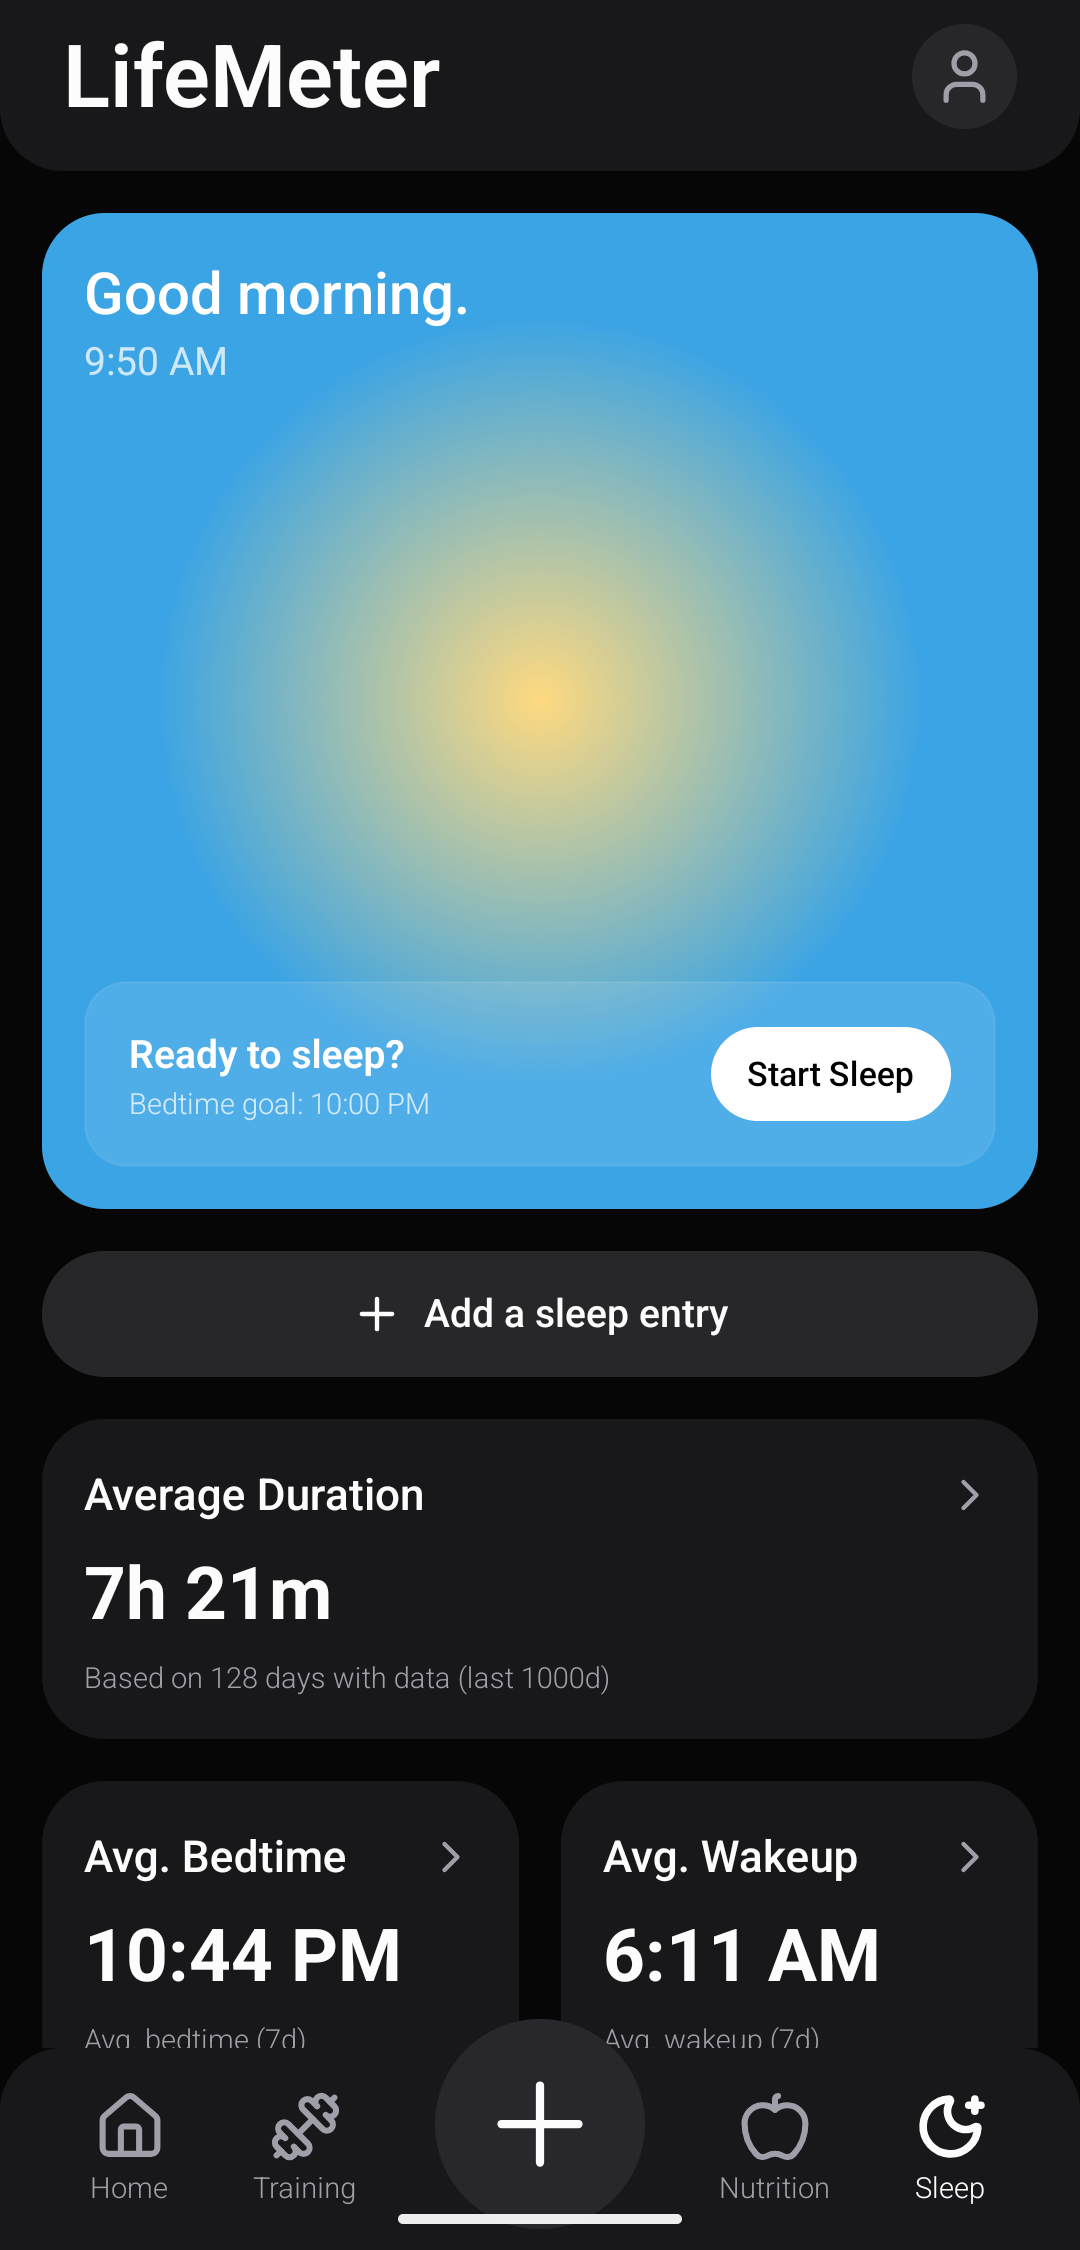
\includegraphics[width=\textwidth]{asset/img/screens/sleep.png}
    % \Screenshot{sleep.png}
    \caption{Modul spánku -- přehled a~záznam}
    \label{fig:screen-sleep}
  \end{minipage}
  \hfill
  \begin{minipage}{0.46\textwidth}
    \centering
    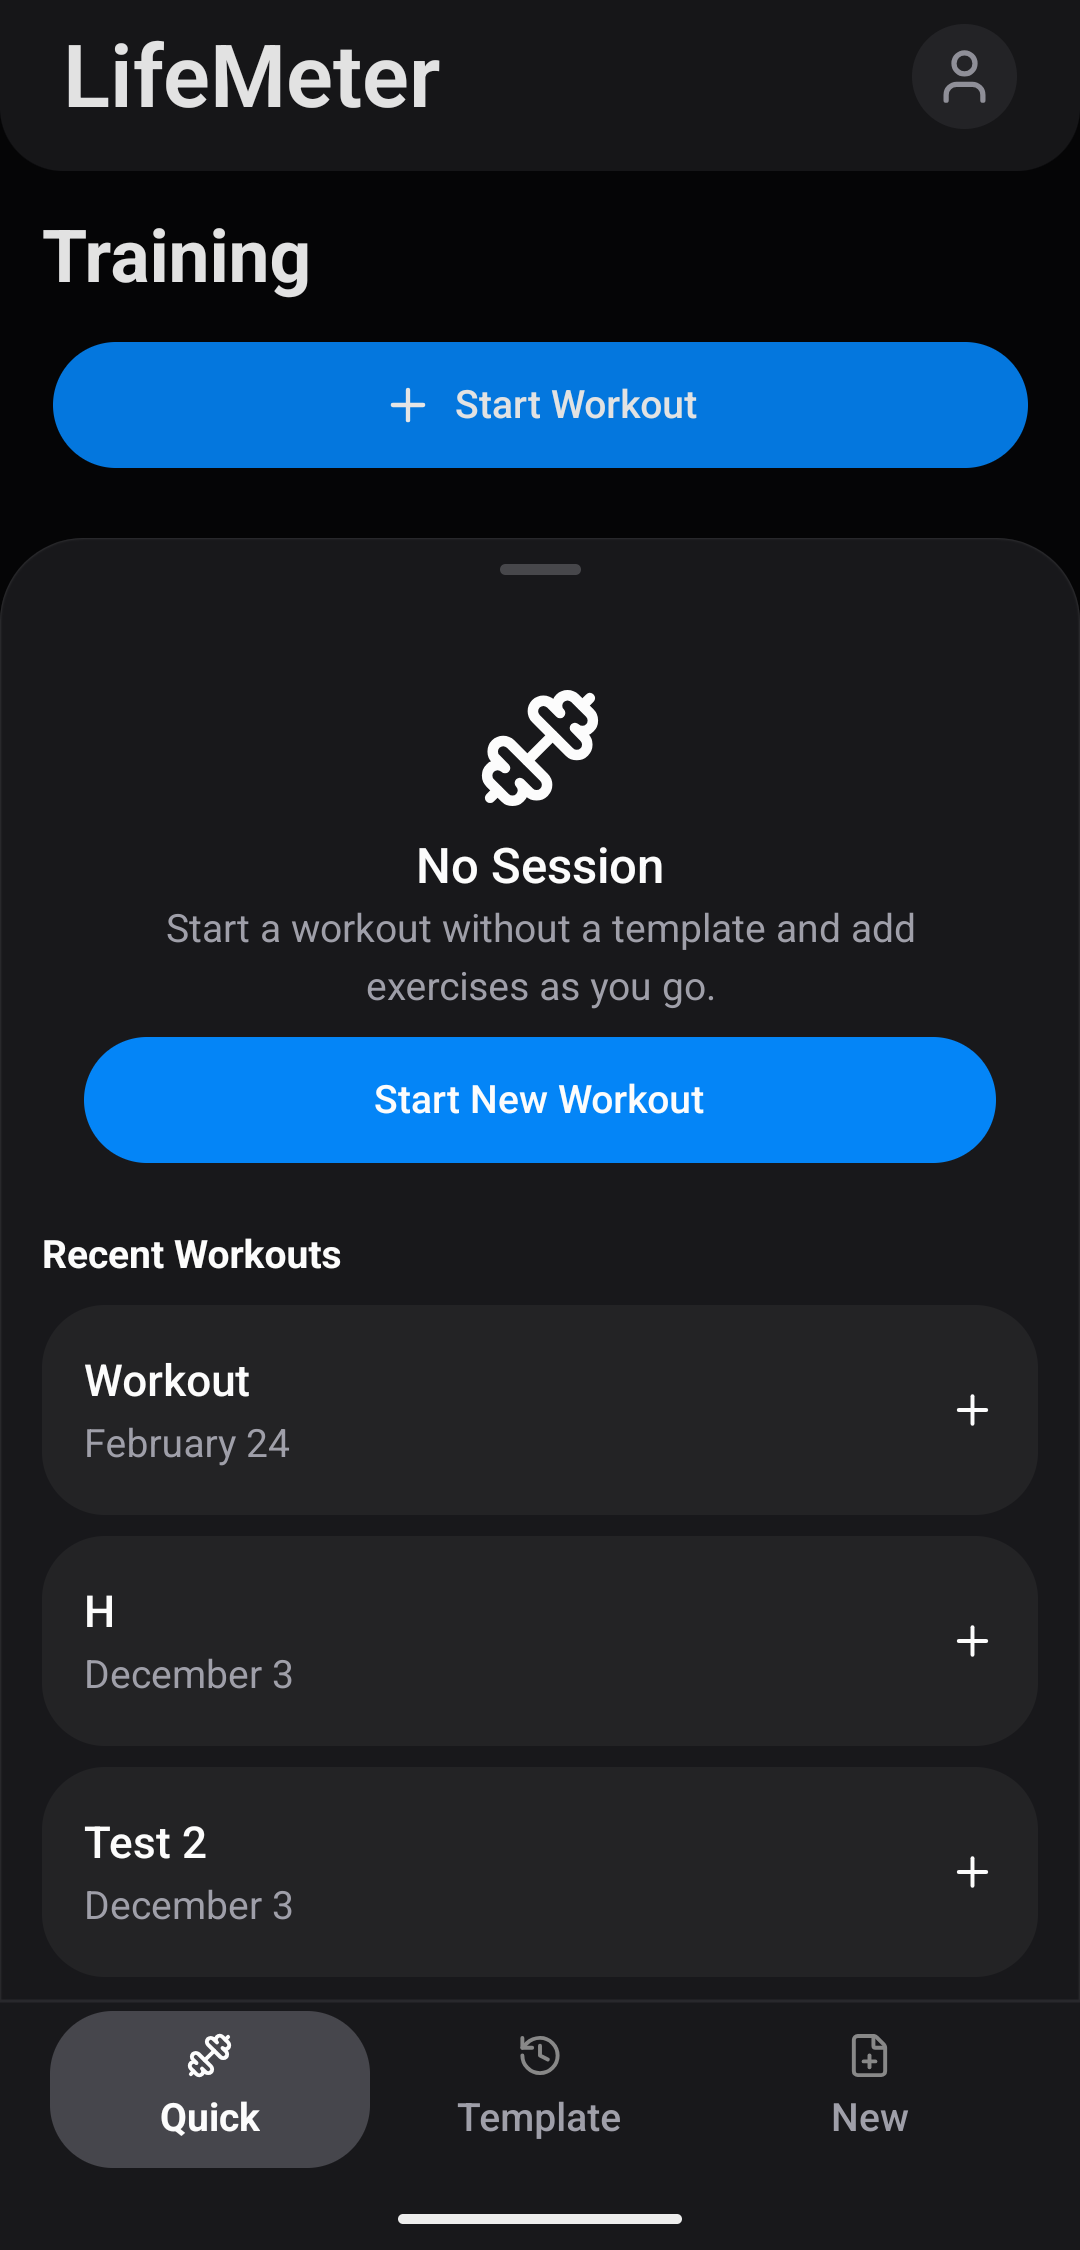
\includegraphics[width=\textwidth]{asset/img/screens/training.png}
    % \Screenshot{training.png}
    \caption{Modul tréninku -- aktivní trénink se sériemi}
    \label{fig:screen-training}
  \end{minipage}
\end{figure}

\begin{figure}[H]
  \centering
  \begin{minipage}{0.46\textwidth}
    \centering
    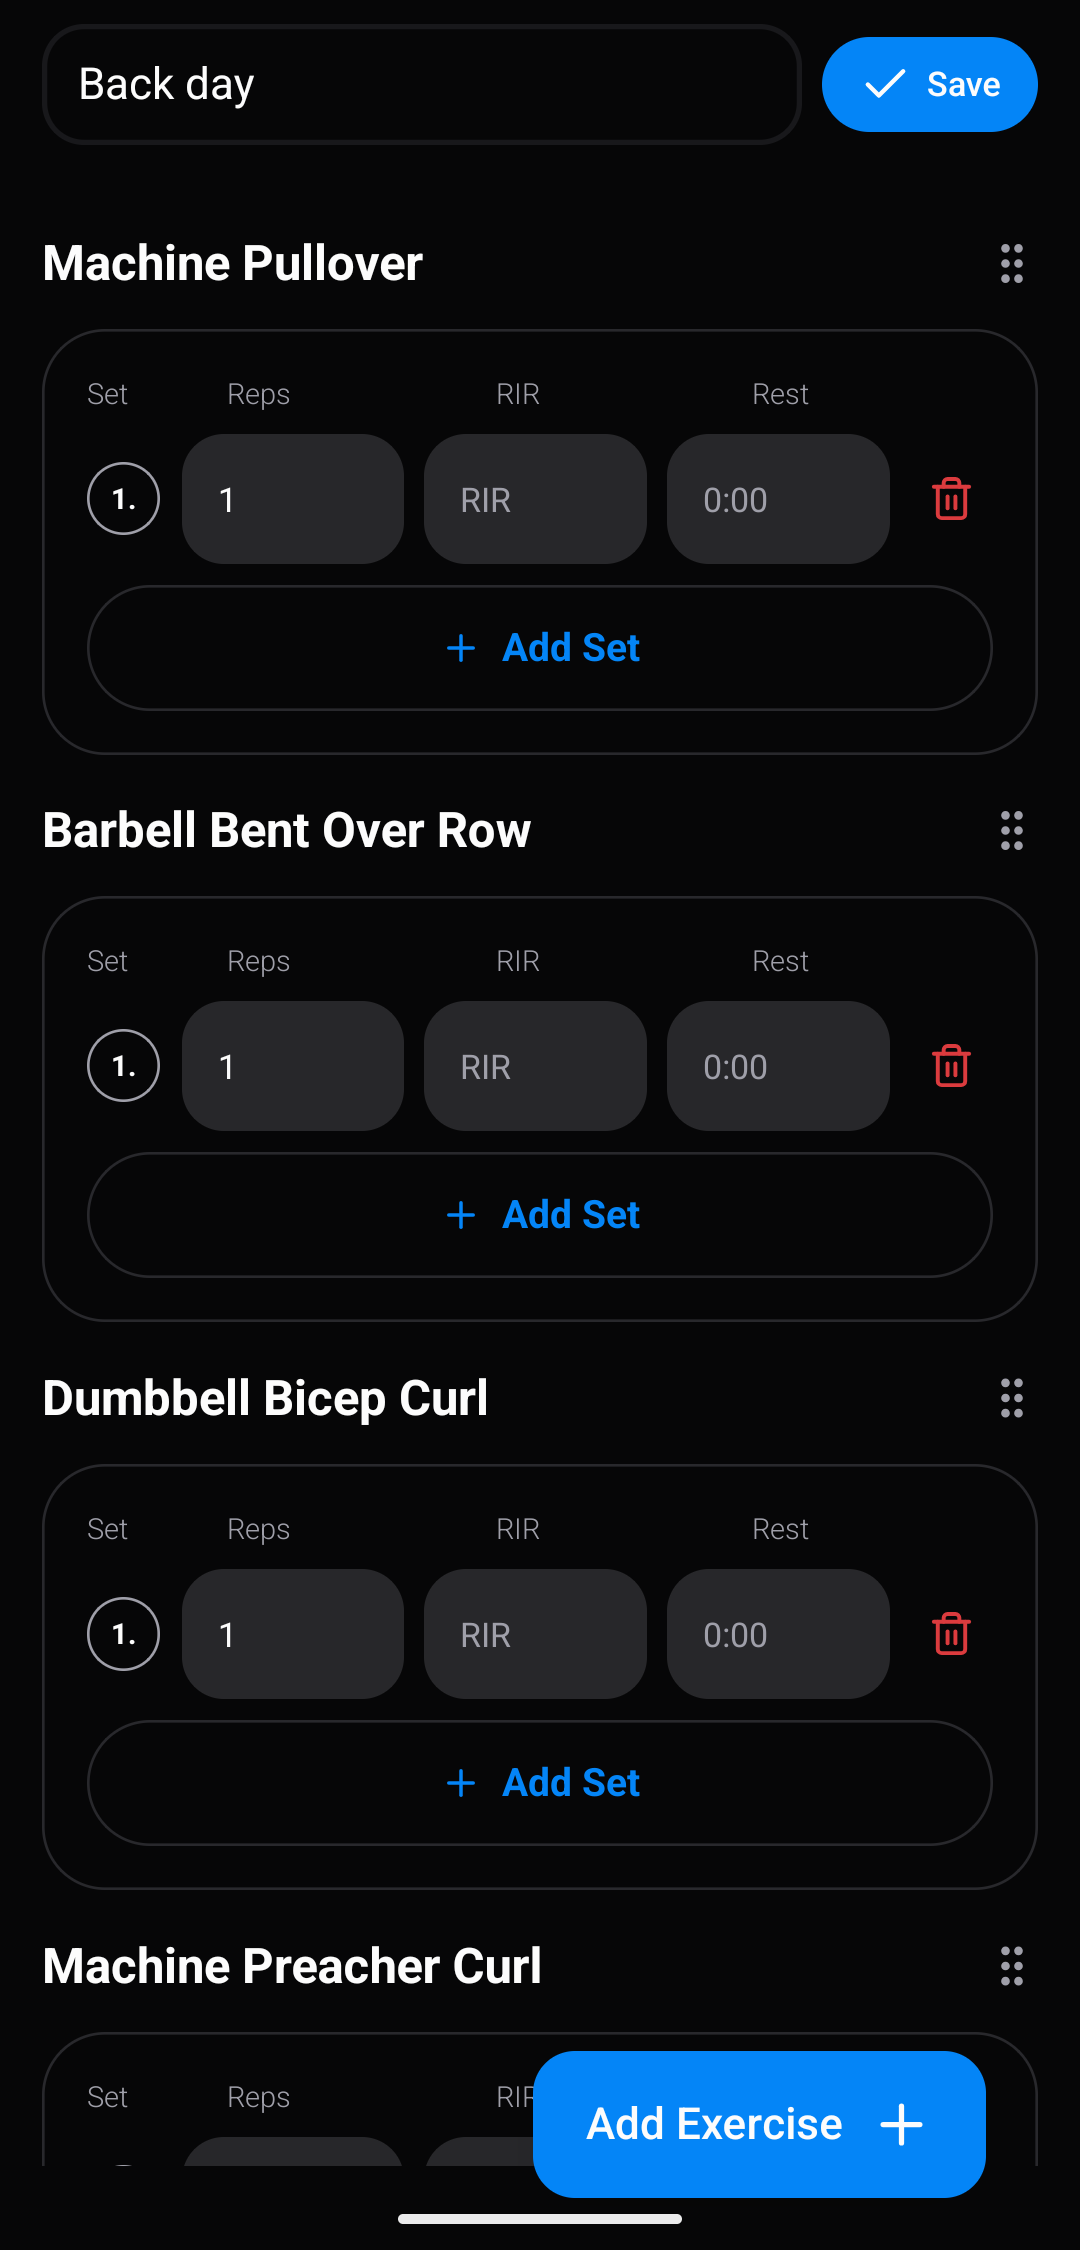
\includegraphics[width=\textwidth]{asset/img/screens/template-builder.png}
    % \Screenshot{template-builder.png}
    \caption{Sestavení tréninkové šablony}
    \label{fig:screen-template}
  \end{minipage}
  \hfill
  \begin{minipage}{0.46\textwidth}
    \centering
    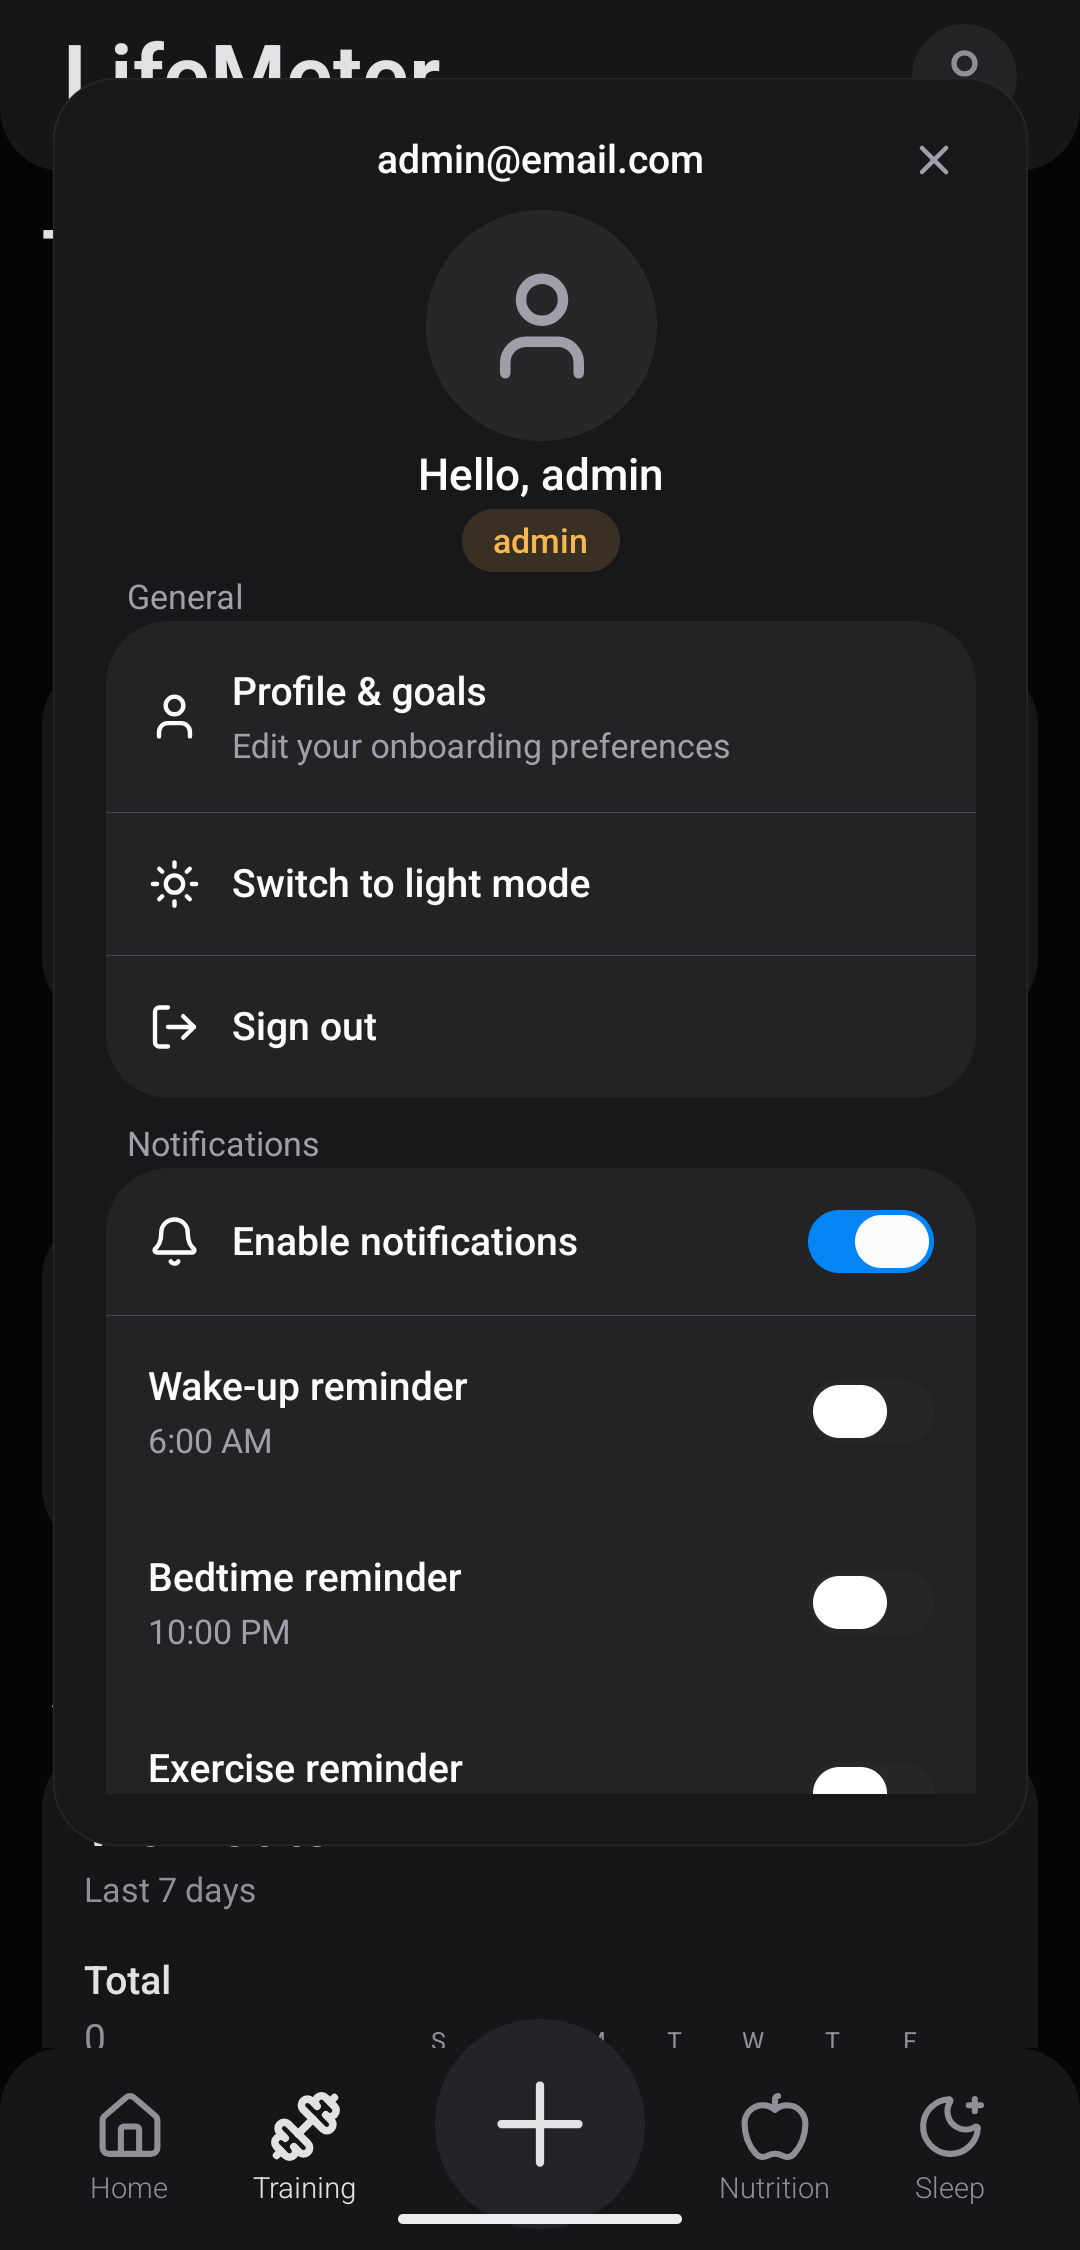
\includegraphics[width=\textwidth]{asset/img/screens/settings.png}
    % \Screenshot{settings.png}
    \caption{Nastavení -- notifikace a~zdravotní integrace}
    \label{fig:screen-settings}
  \end{minipage}
\end{figure}

% ------------------------------------------------------------------
\section{Testování}
% ------------------------------------------------------------------

Aplikace byla průběžně testována ručně na fyzickém zařízení se systémem
Android~16 (Google Pixel 8). Testování se zaměřilo na správnost
ukládání a~zobrazování dat ve všech třech sledovaných doménách
(výživa, spánek, trénink), funkčnost offline fronty při vypnutém
datovém připojení, správné odeslání zařazených požadavků po jeho
obnovení a~správnost výpočtů makronutrientních cílů.

Dále bylo provedeno uživatelské testování s~testovacími uživateli,
kteří aplikaci používali po dobu několika dní v~běžném provozu.
Na základě jejich zpětné vazby byly provedeny úpravy uživatelského
rozhraní -- zejména zjednodušení průvodce onboardingem a~přidání
možnosti přeskočit volitelné položky tělesné kompozice.
